\begin{figure}[H]
	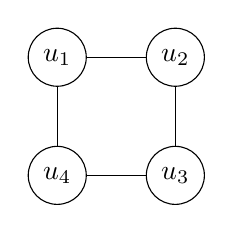
\begin{tikzpicture}[node distance={15mm}, main/.style = {draw, circle}]
		\node[main] (1) {$u_1$};
		\node[main] (2) [right of=1] {$u_2$};
		\node[main] (3) [below of=2] {$u_3$};
		\node[main] (4) [left of=3] {$u_4$};
		\draw (1) -- (2);
		\draw (2) -- (3);
		\draw (3) -- (4);
		\draw (4) -- (1);
	\end{tikzpicture}
	\hspace{3cm}
	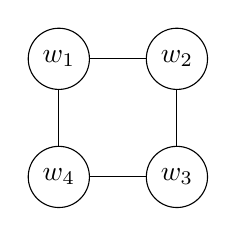
\begin{tikzpicture}[node distance={15mm}, main/.style = {draw, circle}]
		\node[main] (1) {$w_1$};
		\node[main] (2) [right of=1] {$w_2$};
		\node[main] (3) [below of=2] {$w_3$};
		\node[main] (4) [left of=3] {$w_4$};
		\draw (1) -- (2);
		\draw (2) -- (3);
		\draw (3) -- (4);
		\draw (4) -- (1);
	\end{tikzpicture}
	\centering
	\caption{Structure $\mathfrak{G}_2$, consisting of two cycles of length $4$.}
\end{figure}